%%%%%%%%%%%%%%%%%%%%%%%%%%%%%%%%%%%%%%%%%%%%%%%%%%%%%%%%%%%%%%%%%%%%%%%%%%%%%%%%
% Лабораторная работа 1 : Испытание на растяжение.
% Выполнили             : Баталов Семен, Хайретдинова Диана, 2021.
%%%%%%%%%%%%%%%%%%%%%%%%%%%%%%%%%%%%%%%%%%%%%%%%%%%%%%%%%%%%%%%%%%%%%%%%%%%%%%%%

\documentclass[12pt, a4paper]{article}
\usepackage[left=2cm, right=2cm, top=2.5cm, bottom=2.5cm, nohead]{geometry}
\usepackage{graphicx}
\usepackage[utf8]{inputenc}
\usepackage[english, russian]{babel}
\usepackage{indentfirst}
\usepackage{amsmath}
\usepackage{longtable}
\usepackage{multirow}
\usepackage{array}
\usepackage{rotating}
\usepackage{subcaption}
\graphicspath{{./Figures/}}

\begin{document}
    
    \newcolumntype{M}[1]{>{\centering\arraybackslash}m{#1}}
    \renewcommand{\arraystretch}{1.4}
    
    \begin{center}
        \large{Санкт-Петербургский Государственный Университет} \\
        \large{Saint-Petersburg State University}\\
        \hfill \break
        \hfill \break
        \hfill \break
        \hfill \break
        \hfill \break
        \hfill \break
        \hfill \break
        \large{Кафедра теории упругости} \\
        \hfill \break
        \hfill \break
        \large{\textbf{ОТЧЕТ}} \\
        \large{\textbf{По лабораторной работе 1}} \\
        \large{<<Испытание на растяжение>>} \\
        \hfill \break
        \hfill \break
        \hfill \break
        \large{По дисциплине} \\
        \large{<<Лабораторный практикум, лабораторная работа>>} \\
    \end{center}
    
    \hfill \break
    \hfill \break
    \hfill \break
    \hfill \break
    \hfill \break
    \hfill \break
    
    \begin{flushright} 
        \large{Выполнили:} \\
        \hfill \break
        \large{Баталов С. А.} \\
        \large{Хайретдинова Д. Д.} \\
    \end{flushright}
    
    \hfill \break
    \hfill \break
    \hfill \break
    \hfill \break
    \hfill \break
    \hfill \break
    
    \begin{center} 
        \large{Санкт-Петербург} \\
        \large{2021} \\
    \end{center}
    
    \thispagestyle{empty}
    \newpage
    \sloppy
    
    \section{Цель работы}
    
    При малых деформациях и нагрузках почти все материалы обнаруживают свойство упругости, то есть деформации образца обратимы и исчезают после снятия нагрузки. Многие материалы подчиняются при этом закону Гука, то есть удлинение образца прямо пропорционально приложенной нагрузке. При больших нагрузках деформации становятся необратимыми, и начинают работать сложные механизмы развития деформаций. Изучение закономерностей поведения материалов за пределами упругости очень важно для практики, так как оно дает ответ на вопрос о допустимых напряжениях в деталях из данного материала. В данной работе испытываются металлические образцы при комнатной температуре, когда основным механизмом развития деформаций за пределами упругости является пластичность.
    
    В данной лабораторной работе производится испытание образцов на растяжение с деформациями за пределами упругости. Строятся условная и истинная диаграммы растяжения и находятся механические характеристики материалов.
    
    \newpage
    
    \section{Характеристики напряженно-деформированного состояния образца}
    
    Рассмотрим стержень длины $l_{0}$ с площадью поперечного сечения $F_{0}$. Пусть стержень растягивается силой $P$ и при этом удлиняется на $\Delta l$. При удлинении стержня происходит его поперечное сужение, поэтому площадь его поперечного сечения становится равной $F < F_{0}$. Условным напряжением $\sigma$ называют отношение нагрузки к первоначальной площади поперечного сечения:
    
    \begin{equation}
        \sigma = \frac{P}{F_{0}}.
        \label{eq1}
    \end{equation}
    
    Истинным напряжением называют величину $S$~--~отношение нагрузки к текущей площади поперечного сечения, рассчитывается по формуле:
    
    \begin{equation}
        S = \frac{P}{F}.
        \label{eq2}
    \end{equation}
    
    Поле деформаций в образце характеризуется относительным удлинением образца и относительным сужением образца, рассчитываются соответственно:
    
    \begin{equation}
        \epsilon = \frac{\Delta l}{l_{0}} \cdot 100 \%, \qquad
        \psi = \frac{F_{0} - F}{F_{0}} \cdot 100 \%.
        \label{eq3}
    \end{equation}
    
    В формулах (\ref{eq3}) изменение длины и площади поперечного сечения относятся к первоначальным значениям длины и площади сечения. Для характеристики больших деформаций по аналогии с истинным напряжением целесообразно ввести истинные удлинения и истинные сужения:
    
    \begin{equation}
        \begin{aligned}
            de &= \frac{dl}{l} \quad \Rightarrow \quad e = \int_{l_{0}}^{l} \frac{dl}{l} = ln \Big (\frac{l}{l_{0}} \Big ) = ln(1 + \epsilon), \\
            d\overline{\psi} &= -\frac{dF}{F} \quad \Rightarrow \quad \overline{\psi} = \int_{F}^{F_{0}} \frac{dF}{F} = ln \Big (\frac{F_{0}}{F} \Big ).
        \end{aligned}
        \label{eq4}
    \end{equation}
    
    В отличие от относительного удлинения $\epsilon$, логарифмическая деформация обладает свойством аддитивности. Кроме того, формулой (\ref{eq4}) можно пользоваться и при малых деформациях: разлагая логарифмы в ряд и удерживая первый член, в этом случае найдём, что $e \approx \epsilon$.
    
    В нашей задаче сечение стержня представляет из себя круг диаметра $d$. Расчет площади $F$ поперечного сечения в таком случае производится по формуле:
    
    \begin{equation}
        F = \frac{\pi \cdot d^{2}}{4}.
        \label{eq5}
    \end{equation}
    
    \newpage
    
    \section{Описание аппаратуры}
    
    \subsection{Машина ИМ-4Р}
    
    Машина ИМ-4Р предназначена для испытания цилиндрических и плоских образцов на растяжение прямым нагружением. Кроме того, при помощи специальных приспособлений можно проводить испытания на сжатие, изгиб и срез. Машина позволяет прикладывать к образцу нагрузку до 4~т. В процессе испытания автоматически строится диаграмма в координатах <<нагрузка–деформация>>.
    
    \begin{figure}[h]
        \centering
        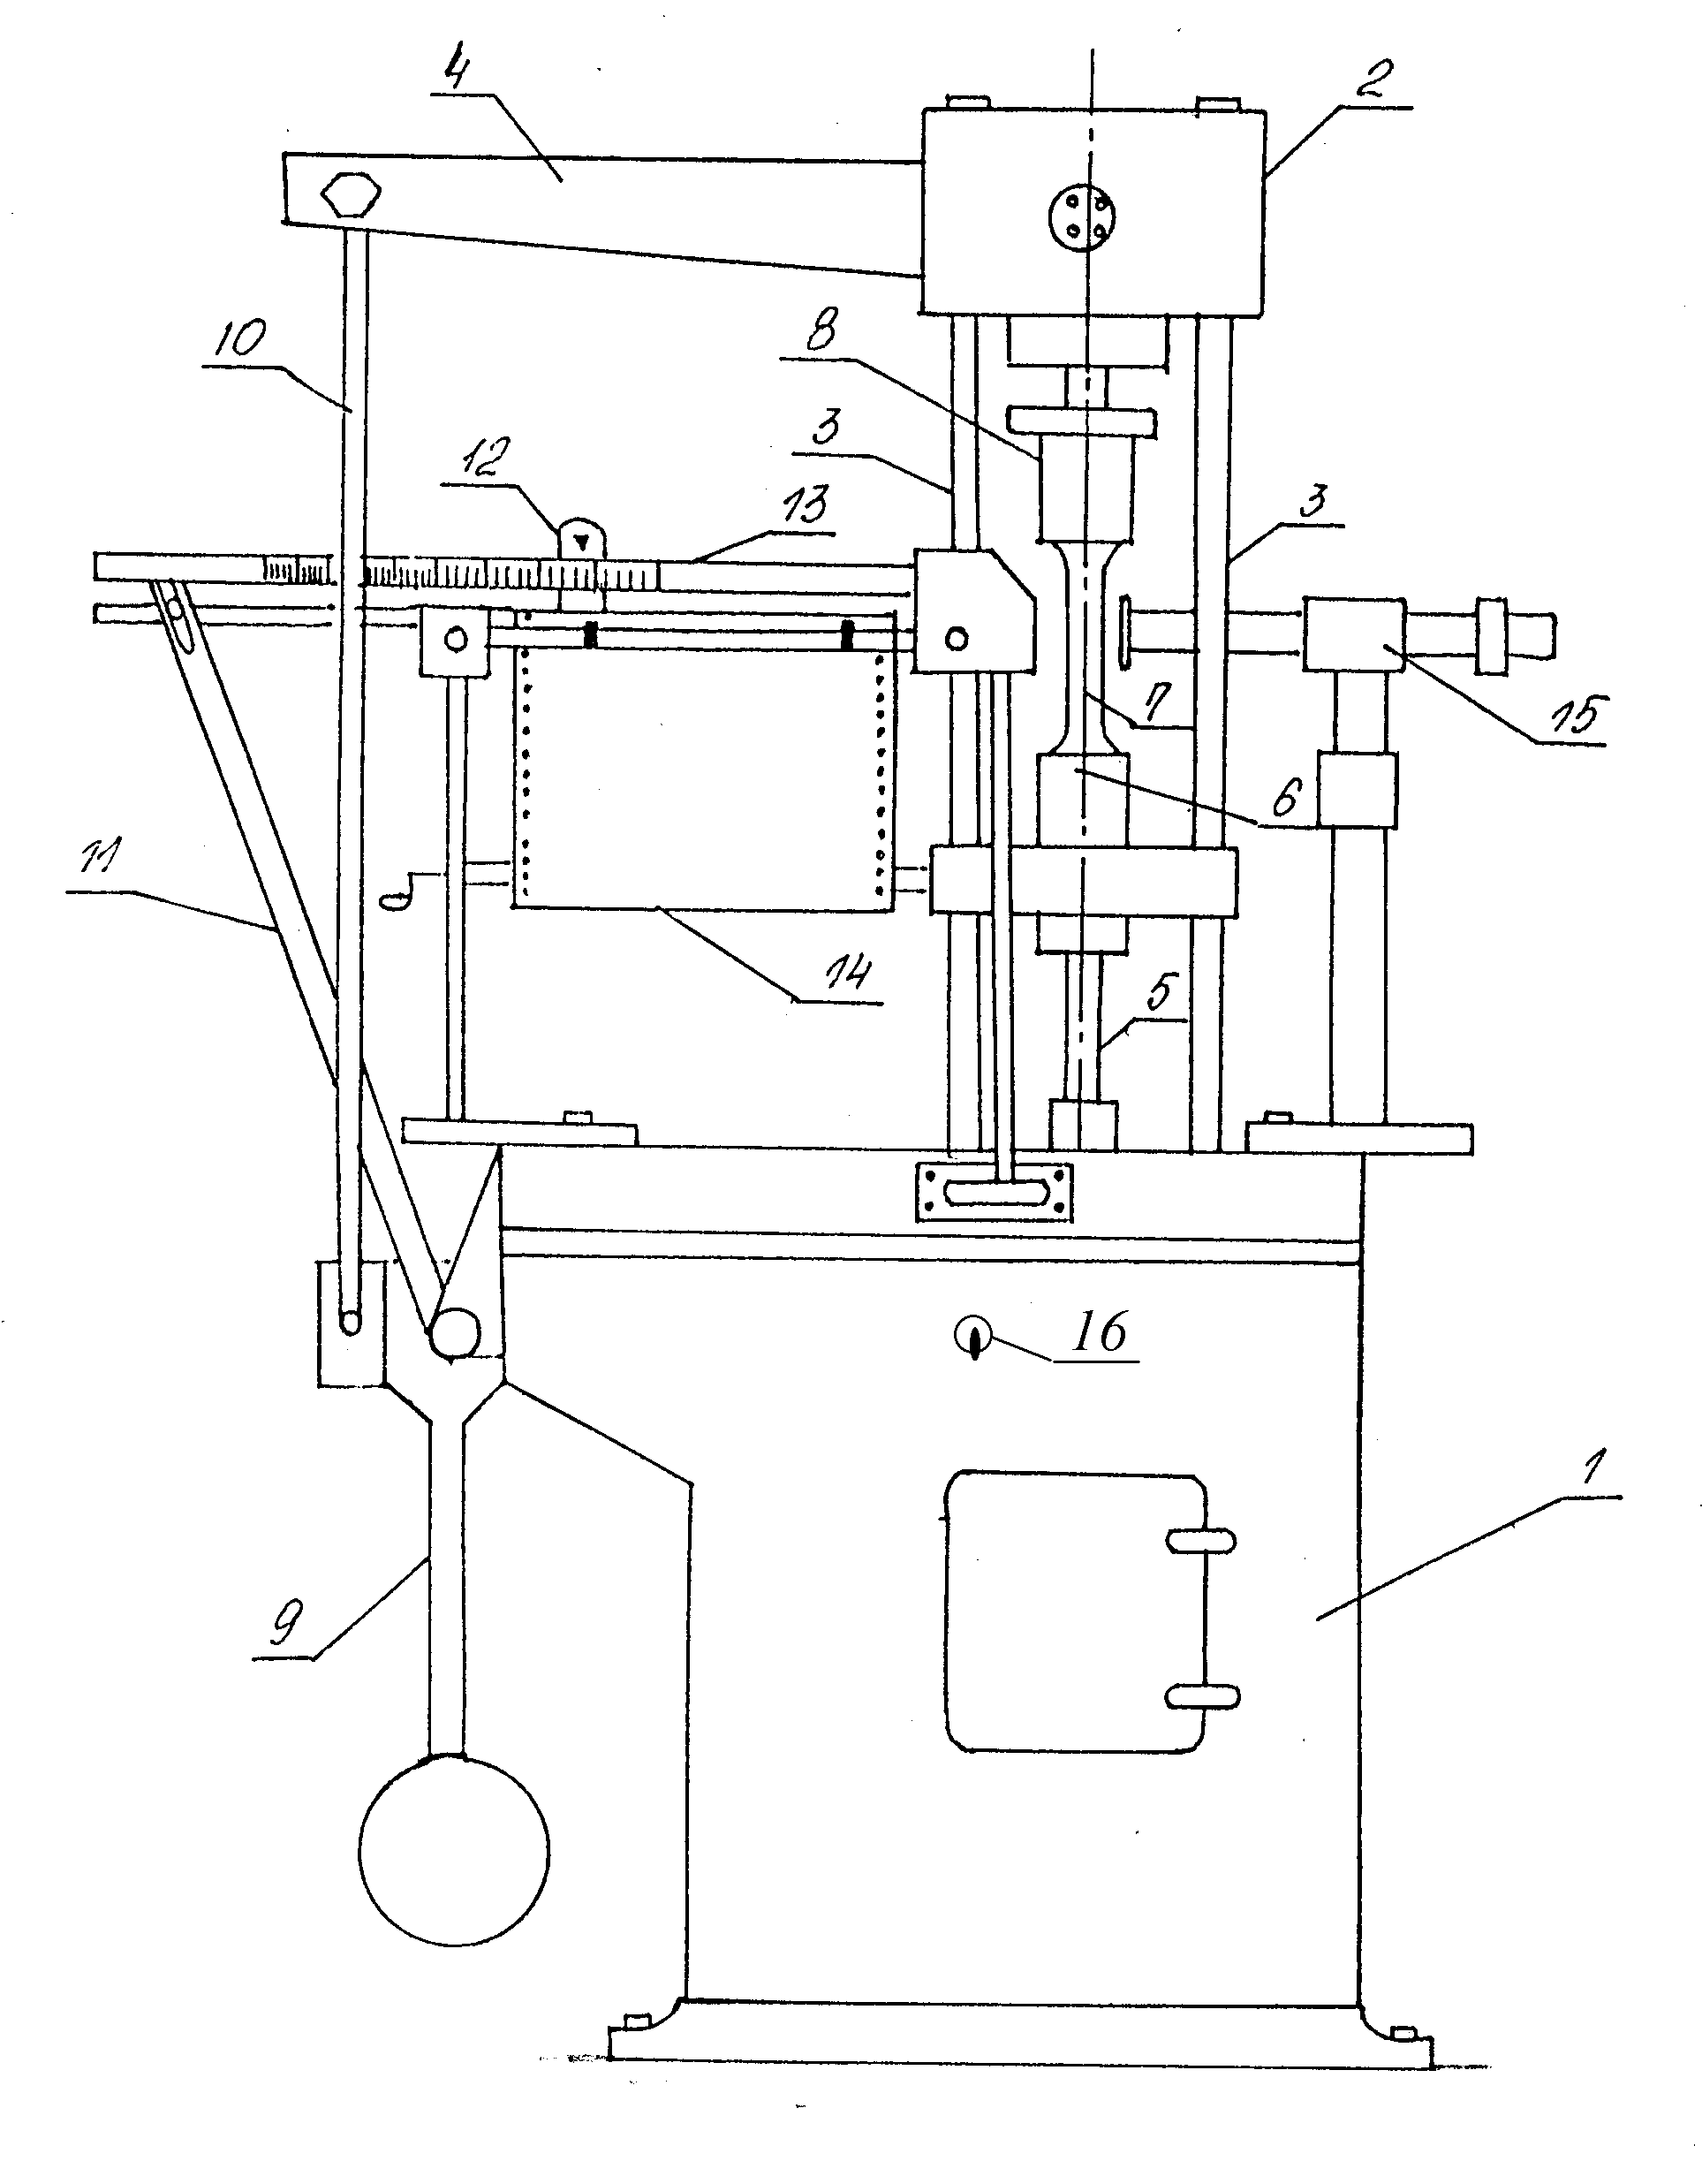
\includegraphics[width = 10cm]{image_1.png}
        \caption{Машина ИМ-4Р.}
        \label{im1}
    \end{figure}
    
    Устройство машины показано на рис.~\ref{im1}. Машина состоит из нагружающего и измерительного механизмов, смонтированных на станине. Станина состоит из нижней (1) и верхней (2) частей, соединенных четырьмя вертикальными стойками (3). В нижней части станины установлен электродвигатель.
    
    При работе электродвигателя движение через коробку передач передается шпинделю (5). Движение шпинделя вниз соответствует рабочему ходу (нагрузке), а движение вверх~--~холостому ходу (разгрузке). На шпинделе установлен нижний захват (6) для крепления образца (7). верхний конец образца крепится в захвате (8), связанном с механизмом силоизмерителя.
    
    Силоизмерительный механизм состоит из рычага (4), связанного тягой (10) с маятником (9). Отклонение маятника через поводок (11) передается на каретку (12) самописца.
    
    Машина снабжена самописцем (14), позволяющим в процессе испытания строить диаграмму «нагрузка~--~абсолютное удлинение». Валик самописца связан через систему шестерен со шпинделем нагружающего механизма, поэтому по продольной оси диаграммы откладывается перемещение нижнего захвата (то есть абсолютное удлинение образца). Перо самописца укреплено в каретке (12), соединенной с силоизмерителем. Таким образом, по поперечной оси диаграммы откладывается есть действующее на образец усилие. Цена деления самописца: 1~мм диаграммы по продольной оси соответствует удлинению образца на 0.01~мм, 1~мм диаграммы по поперечной оси соответствует нагрузке 10~кг. Для измерения диаметра образца в процессе испытания служит окуляр–микрометр (15).
    
    \subsection{Окуляр–микрометр}
    
    Окуляр–микрометр (рис.~\ref{im2}) состоит из зрительной трубки (1), которую можно поднимать и опускать по вертикали рифленой гайкой (3) и наводить по горизонтали винтом (5). Замеры выполняются по шкале (а) и барабану (2). Для удобства наблюдения образец подсвечивается лампой, снабженной металлическими шторками.
    
    \begin{figure}[h]
        \centering
        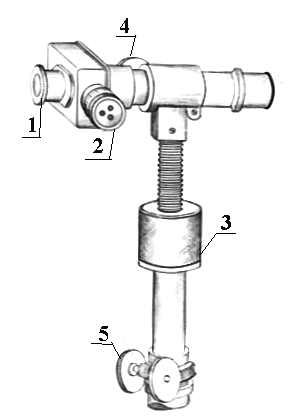
\includegraphics[width = 13cm]{image_2.png}
        \caption{Окуляр–микрометр.}
        \label{im2}
    \end{figure}
    
    Для снятия показаний с окуляр-микрометра требуется вычислить коэффициент $K$ по следующей формуле:
    
    \begin{equation}
        K = \frac{d_{0}}{d_{0}'}
        \label{eq6}
    \end{equation}
    
    Здесь диаметр $d_{0}'$~--~диаметр, измеренный окуляр–микрометром. Теперь диаметр образца в момент времени $t$ будет вычисляться по формуле:
    
    \begin{equation}
        d_{t} = K \cdot d_{t}'
        \label{eq7}
    \end{equation}
    
    \newpage
    
    \section{Эксперимент}
    
    Работа проводилась на испытательной установке ИМ-4Р. Производилась деформация железного стержня (рис.~\ref{im3}), начальные размеры которого равны $d_{0} = 5.4~\text{мм}$ и $l_{0} = 43~\text{мм}$. Важно отметить, что все вычисления и построения производились с помощью пакета Matlab, с исходным кодом программы можно ознакомиться отдельно.
    
    \begin{figure}[h]
        \centering
        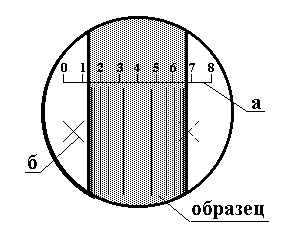
\includegraphics[width = 10cm]{image_3.png}
        \caption{Эскиз стержня.}
        \label{im3}
    \end{figure}
    
    Регистрация диаметра стержня в процессе нагружения осуществлялась окуляр-микрометром (все результаты измерений представлены в таблице~\ref{tb2}). Для снятия показаний с данного прибора нужно использовать формулу (\ref{eq7}), требуется найти коэффициент пропорциональности по формуле (\ref{eq6}), и для предоставленного окуляр-микрометра он равен $K = 0.63$. Составим таблицу начальных данных:
    
    \begin{table}[h]
        \centering
        \caption{\centering Начальные данные.}
        \begin{tabular}{| M{2cm} | M{2cm} | M{2cm} | M{2cm} | M{2cm} |}
            \hline
            \multicolumn{2}{|c|}{$d_{0}$} & \multicolumn{2}{c|}{$l_{0}$} & \multirow{2}{*}{$K$} \\
            \cline{1-4}
            \multicolumn{2}{|c|}{мм} & \multicolumn{2}{c|}{мм} & \\
            \hline
            5.3 & \multirow{3}{*}{5.4} & 42.8 & \multirow{3}{*}{43} & \multirow{3}{*}{0.63} \\
            5.6 &  & 43.0 & & \\
            5.2 &  & 43.2 & & \\
            \hline
        \end{tabular}
        \label{tb1}
    \end{table}
    
    \begin{figure}[h]
        \centering
        \begin{subfigure}{.5\textwidth}
            \centering
            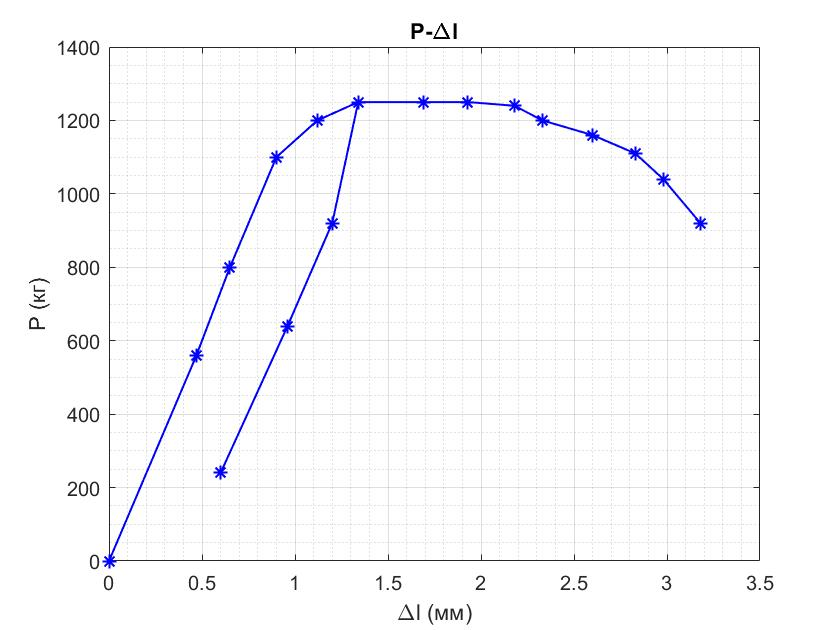
\includegraphics[width = 9cm]{fig_1.jpg}
            \caption{Координаты $P-\Delta l$.}
            \label{fig::fig1}
        \end{subfigure}%
        \begin{subfigure}{.5\textwidth}
            \centering
            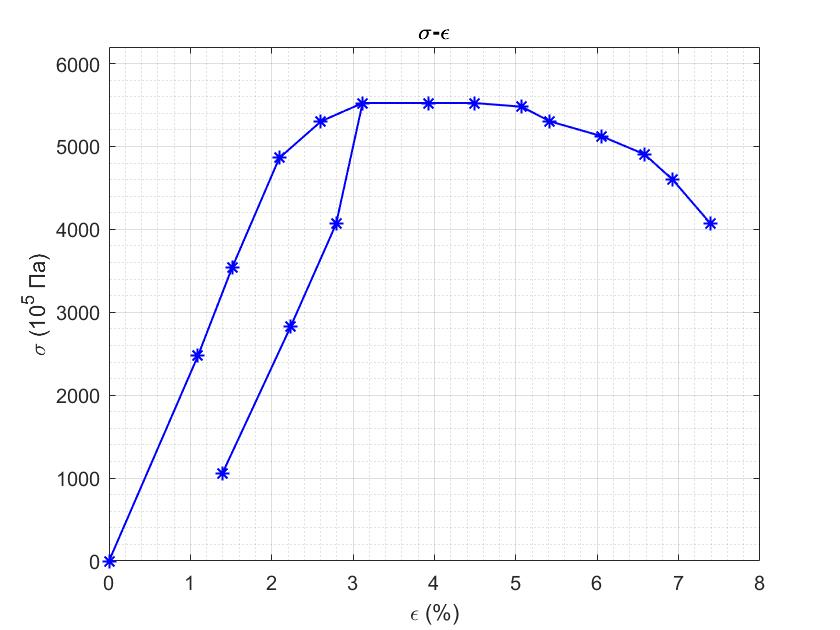
\includegraphics[width = 9cm]{fig_2.jpg}
            \caption{Координаты $\sigma-\epsilon$.}
            \label{fig::fig2}
        \end{subfigure}
        \begin{subfigure}{.5\textwidth}
            \centering
            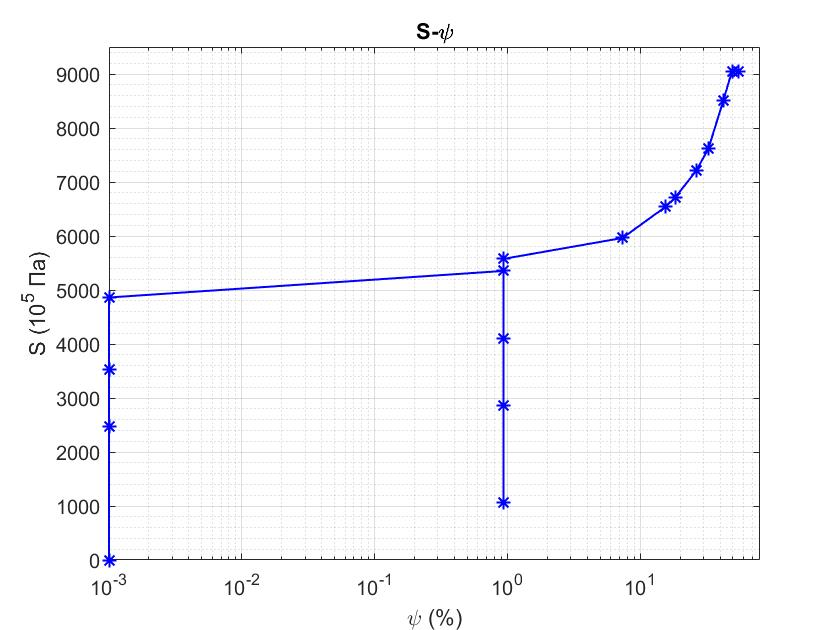
\includegraphics[width = 9cm]{fig_3.jpg}
            \caption{Координаты $S-\psi$.}
            \label{fig::fig3}
        \end{subfigure}%
        \begin{subfigure}{.5\textwidth}
            \centering
            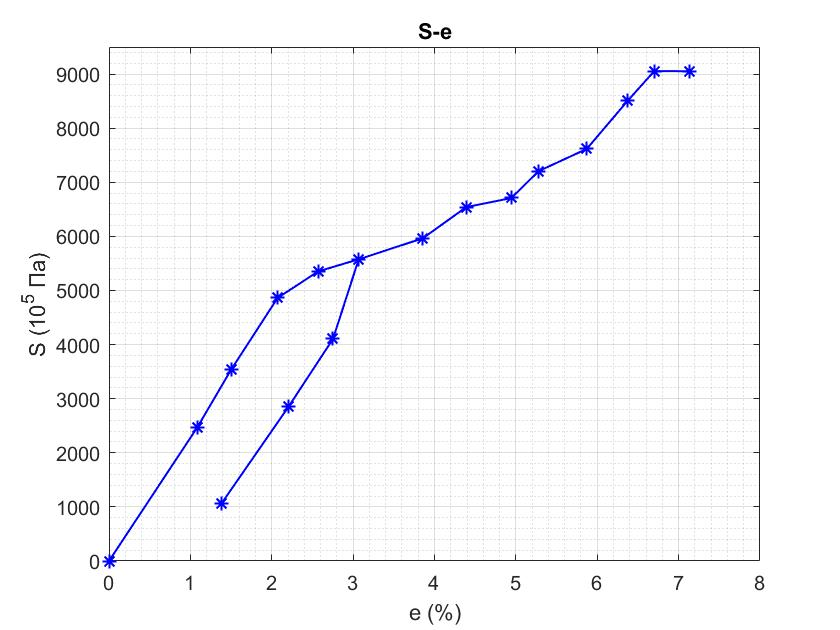
\includegraphics[width = 9cm]{fig_4.jpg}
            \caption{Координаты $S-e$}
            \label{fig::fig4}
        \end{subfigure}
        \caption{Диаграммы растяжения в различных координатах.}
        \label{fig}
    \end{figure}
    
    \newpage
    
    \begin{sidewaystable}
        \centering
        \caption{\centering Результаты измерений и расчеты.}
        \begin{tabular}[p]{| M{1cm} | M{1.5cm} | M{1.5cm} | M{1.5cm} | M{1.5cm} | M{1.5cm} | M{1.5cm} | M{1.5cm} | M{1.5cm} | M{1.5cm} | M{1.5cm} | M{1.5cm} |}
            \hline
            \multirow{2}{*}{№} & $P$ & $\Delta l$ & $d'$ & $d$ & F & $\sigma$ & S & $\epsilon$ & $\psi$ & e & $\overline{\psi}$ \\
            \cline{2-12}
            & кг & мм & мм & мм & $\text{мм}^2$ & $\text{кг} / \text{см}^2$ & $\text{кг} / \text{см}^2$ & \% & \% & \% & \% \\
            \hline
            1 & 0 & 0 & 8.52 & 5.4 & 22.6 & 0 & 0 & 0 & 0 & 0 & 0 \\
            2 & 560 & 0.47 & 8.52 & 5.4 & 22.6 & 2475 & 2475 & 1.1 & 0 & 1.1 & 0 \\
            3 & 800 & 0.65 & 8.52 & 5.4 & 22.6 & 3535 & 3535 & 1.5 & 0 & 1.5 & 0 \\
            4 & 1100 & 0.9 & 8.52 & 5.4 & 22.6 & 4861 & 4861 & 2.1 & 0 & 2.1 & 0 \\
            5 & 1200 & 1.12 & 8.48 & 5.3 & 22.4 & 5303 & 5353 & 2.6 & 0.9 & 2.6 & 0.9 \\
            6 & 1250 & 1.34 & 8.48 & 5.3 & 22.4 & 5524 & 5576 & 3.1 & 0.9 & 3.1 & 0.9 \\
            7 & 920 & 1.2 & 8.48 & 5.3 & 22.4 & 4066 & 4104 & 2.8 & 0.9 & 2.8 & 0.9 \\
            8 & 640 & 0.96 & 8.48 & 5.3 & 22.4 & 2828 & 2855 & 2.2 & 0.9 & 2.2 & 0.9 \\
            9 & 240 & 0.6 & 8.48 & 5.3 & 22.4 & 1061 & 1071 & 1.4 & 0.9 & 1.4 & 0.9 \\
            10 & 640 & 0.96 & 8.48 & 5.3 & 22.4 & 2828 & 2855 & 2.2 & 0.9 & 2.2 & 0.9 \\
            11 & 920 & 1.2 & 8.48 & 5.3 & 22.4 & 4066 & 4104 & 2.8 & 0.9 & 2.8 & 0.9 \\
            12 & 1250 & 1.34 & 8.48 & 5.3 & 22.4 & 5524 & 5576 & 3.1 & 0.9 & 3.1 & 0.9 \\
            13 & 1250 & 1.69 & 8.2 & 5.2 & 21 & 5524 & 5964 & 3.9 & 7.4 & 3.9 & 7.7 \\
            14 & 1250 & 1.93 & 7.83 & 4.9 & 19.1 & 5524 & 6541 & 4.5 & 15.5 & 4.4 & 16.9 \\
            15 & 1240 & 2.18 & 7.7 & 4.9 & 18.5 & 5480 & 6709 & 5.1 & 18.3 & 4.9 & 20.2 \\
            16 & 1200 & 2.33 & 7.31 & 4.6 & 16.7 & 5303 & 7204 & 5.4 & 26.4 & 5.3 & 30.6 \\
            17 & 1160 & 2.6 & 6.99 & 4.4 & 15.2 & 5126 & 7616 & 6 & 32.7 & 5.9 & 39.6 \\
            18 & 1110 & 2.83 & 6.47 & 4.1 & 13 & 4905 & 8506 & 6.6 & 42.3 & 6.4 & 55 \\
            19 & 1040 & 2.98 & 6.07 & 3.8 & 11.5 & 4596 & 9055 & 6.9 & 49.2 & 6.7 & 67.8 \\
            20 & 920 & 3.18 & 5.71 & 3.6 & 10.2 & 4066 & 9052 & 7.4 & 55.1 & 7.1 & 80 \\
            \hline
        \end{tabular}
        \label{tb2}
    \end{sidewaystable}
    
\end{document}